\section{Architecture and Design}

In this section we will discuss the specific solutions that we built in order to
achieve our goals, the motivations behind our design decisions, and the
technical challenges we overcame. Our project ended up being divided into a
series of independent components; Bee, our data agent; Hive, responsible for
storage and processing of data; Queen, our web front end; and finally, our iOS
application.

\graphicspath{{./pics/}}
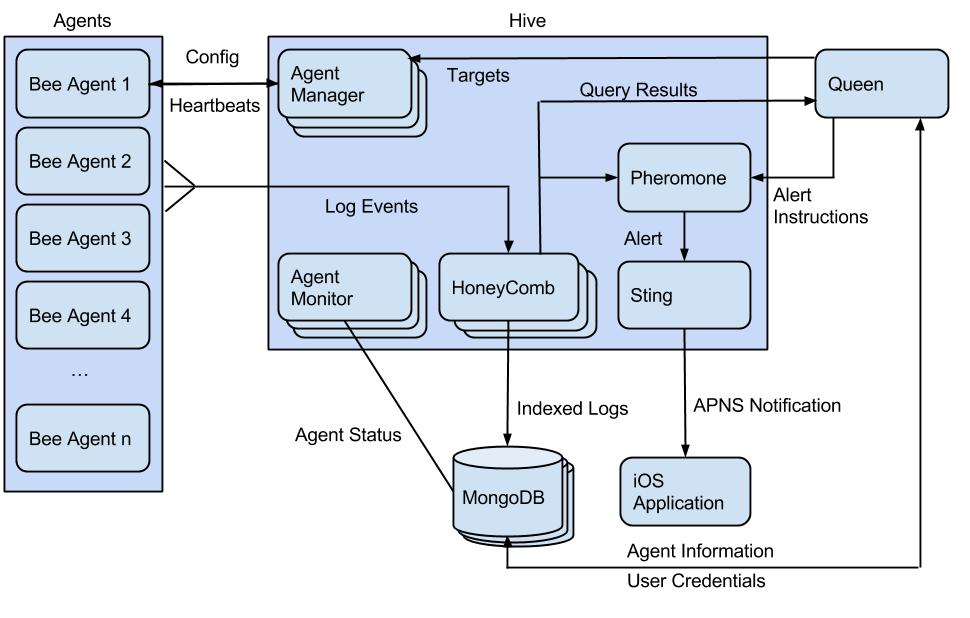
\includegraphics[width=\textwidth, keepaspectratio]{design.jpg}

The key design decision was to build our system in a ‘Process Oriented’ manner.
This meant all components were broken down into small, scalable components. All
state was stored in a central, scalable database, and all communication was
handled by a scalable RabbitMQ\cite{rabbit} messaging exchange. Designing the system in
this way meant that we could leverage these technologies to provide a reliable,
transparently scalable, and real time system.

The reasons for choosing RabbitMQ over other communication paradigms and
technologies, such as REST, were that it would provide automatic distribution of
messages across subscribers, giving us free load balancing and thus scaling. It
would also queue messages in the case of congestion, ensuring reliability, and
behaves in an event driven manner - allowing us to react in real-time to events
across the whole stack.

For the database we opted for MongoDB\cite{mongo}. We decided this was the best option
for the project because of the necessity to have very flexible data structures.
MongoDB stores collections of JSON objects instead of having rigid tables,
allowing for metadata and optional extra fields to be added dynamically to
objects - a feature that we specifically wanted for log entries. Due to the
lack of relations in MongoDB it is also known to scale very well, and because
MongoDB is JSON based like the rest of our stack, we would avoid data
consistency issues as no conversion would need to be performed between
components.
